\documentclass{beamer}
\usepackage[english,russian]{babel}
\usepackage[utf8]{inputenc}
\usepackage{amsmath}
\usepackage{hyperref}
\usetheme{Warsaw}
\usepackage{listings}
\usepackage{xcolor}
\usepackage{tikz}
\usetikzlibrary{graphs}

\lstset{
    frame=tb,
    tabsize=4,
    showstringspaces=false,
    numbers=left,
    commentstyle=\color{green},
    keywordstyle=\color{blue},
    stringstyle=\color{red},
    emph={baz},
    emphstyle=\textbf
}

\begin{document}

\title{Задачи разрешимости логических формул и приложения\newline Лекция 4. Введение в SMT}
\author{Роман Холин}
\institute{Московский государственный университет}
\date{Москва, 2021}

\begin{frame}
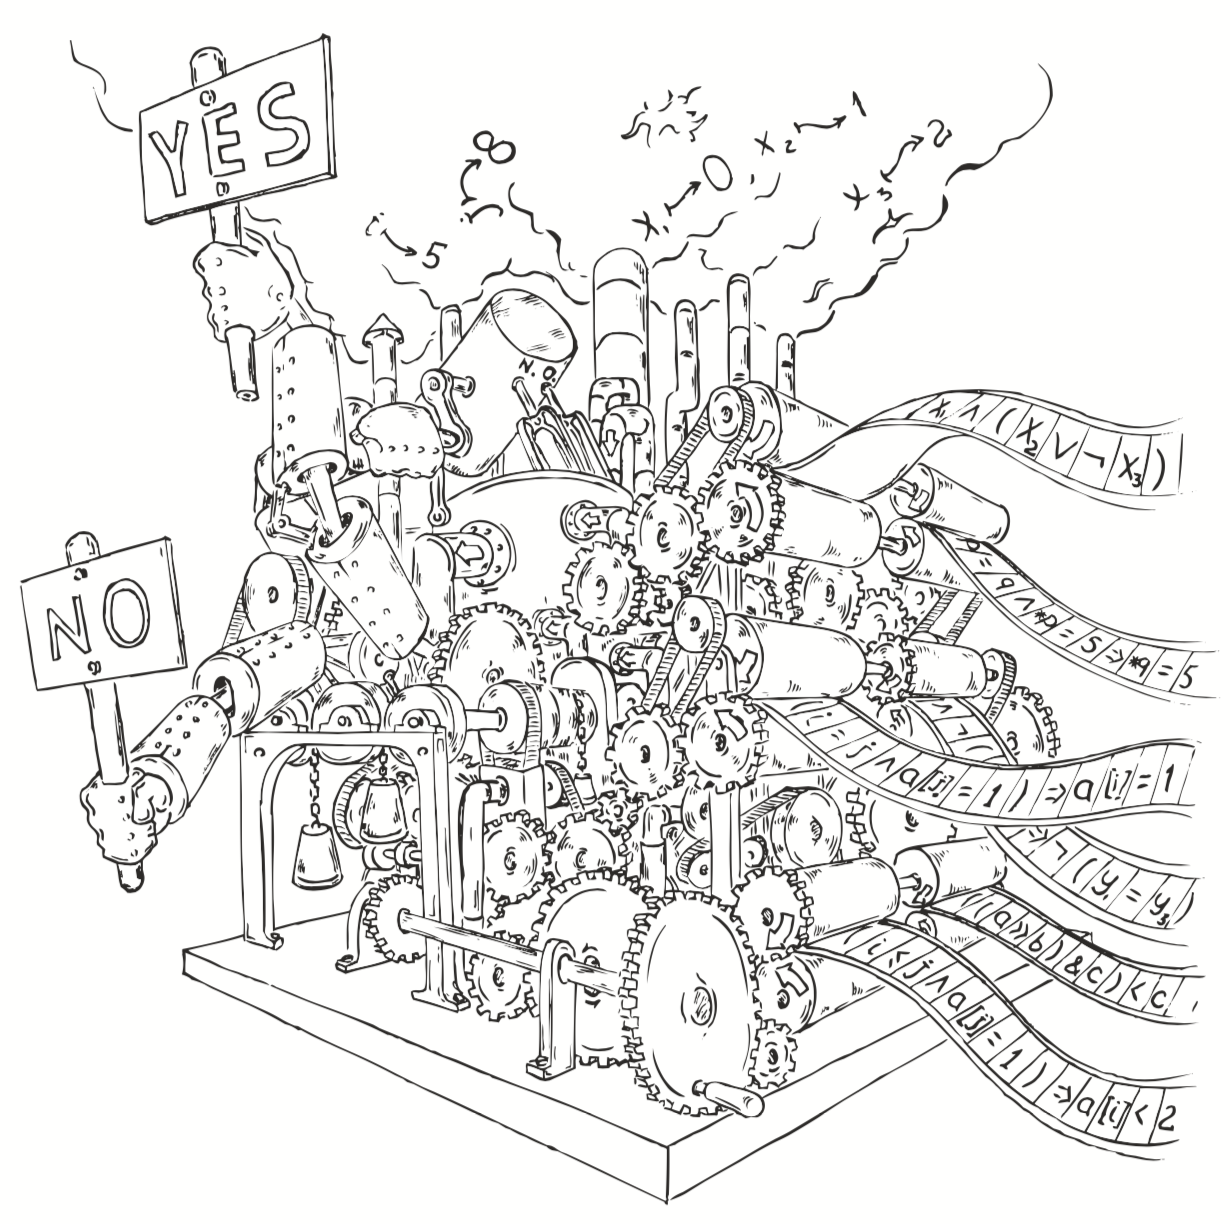
\includegraphics[scale=0.5]{../decision-procedure.png}
\end{frame}

\frame{\titlepage}

\begin{frame}{Определения}
\begin{itemize}
\item $at(\phi)$ - множество атомов в формуле $\phi$
\item $at_i(\phi)$ - некоторый заданный порядок этих атомов
\item Атом $a$ сопоставим с булевой переменной $e(a)$ (такую процедуру будем называть булевское кодирование)
\item $e(t)$ - булева формула, полученную булевым кодированием каждого атома формулы $t$ (такую формулу будем называть
пропозиционным скилетом формулы $t$)
\end{itemize}
\end{frame}

\begin{frame}{Пример}
\begin{itemize}
\item $\phi := x = y \vee x = z$
\item $e(x = y) = b_1$
\item $e(x = z) = b_2$
\item $e(\phi) = b_1 \vee b_2$
\end{itemize}
\end{frame}

\begin{frame}{Определения}
\begin{itemize}
\item $\alpha$ - некоторая (возможно, частичная) оценка формулы $e(\phi)$
\item $\alpha = \{e(at_1) \rightarrow FALSE, e(at_2) \rightarrow TRUE\}$
\item $Th(at_i, \alpha) = at_i$, если $\alpha(at_i) = TRUE$, $\lnot at_i$ иначе
\item $Th(\alpha) = \{Th(at_i, \alpha)| для всех e(at_i), оцененных \alpha\}$
\item $\overline{Th(\alpha)}$ - конъюнкция всех элементов их $Th(\alpha)$
\end{itemize}
\end{frame}

\begin{frame}{Ленивый алгоритм решение SMT задач}
Пусть нам данн алгоритм (назовём его $Deduction$), который может решить $\overline{Th(\alpha)}$
\begin{itemize}
\item Вычислим $B = e(\phi)$
\end{itemize}
\end{frame}

\begin{frame}{Ленивый алгоритм решение SMT задач}
Пусть нам данн алгоритм (назовём его $Deduction$), который может решить $\overline{Th(\alpha)}$
\begin{itemize}
\item Вычислим $B = e(\phi)$
\item Отправим $B$ SAT-решателю
\end{itemize}
\end{frame}

\begin{frame}{Ленивый алгоритм решение SMT задач}
Пусть нам данн алгоритм (назовём его $Deduction$), который может решить $\overline{Th(\alpha)}$
\begin{itemize}
\item Вычислим $B = e(\phi)$
\item Отправим $B$ SAT-решателю
\item Если получили "UNSAT", то возвращаем "UNSAT"
\end{itemize}
\end{frame}

\begin{frame}{Ленивый алгоритм решение SMT задач}
Пусть нам данн алгоритм (назовём его $Deduction$), который может решить $\overline{Th(\alpha)}$
\begin{itemize}
\item Вычислим $B = e(\phi)$
\item Отправим $B$ SAT-решателю
\item Если получили "UNSAT", то возвращаем "UNSAT"
\item Если получили "UNKNOWN", то возвращаем "UNKNOWN"
\end{itemize}
\end{frame}

\begin{frame}{Ленивый алгоритм решение SMT задач}
Пусть нам данн алгоритм (назовём его $Deduction$), который может решить $\overline{Th(\alpha)}$
\begin{itemize}
\item Вычислим $B = e(\phi)$
\item Отправим $B$ SAT-решателю
\item Если получили "UNSAT", то возвращаем "UNSAT"
\item Если получили "UNKNOWN", то возвращаем "UNKNOWN"
\item Если получили некоторую $\alpha$, то вычисляем $Deduction$ от $\overline{Th(\alpha)}$
\end{itemize}
\end{frame}

\begin{frame}{Ленивый алгоритм решение SMT задач}
Пусть нам данн алгоритм (назовём его $Deduction$), который может решить $\overline{Th(\alpha)}$
\begin{itemize}
\item Вычислим $B = e(\phi)$
\item Отправим $B$ SAT-решателю
\item Если получили "UNSAT", то возвращаем "UNSAT"
\item Если получили "UNKNOWN", то возвращаем "UNKNOWN"
\item Если получили некоторую $\alpha$, то вычисляем $Deduction$ от $\overline{Th(\alpha)}$
\item Если получили "SAT", то возвращаем "SAT"
\end{itemize}
\end{frame}

\begin{frame}{Ленивый алгоритм решение SMT задач}
Пусть нам данн алгоритм (назовём его $Deduction$), который может решить $\overline{Th(\alpha)}$
\begin{itemize}
\item Вычислим $B = e(\phi)$
\item Отправим $B$ SAT-решателю
\item Если получили "UNSAT", то возвращаем "UNSAT"
\item Если получили "UNKNOWN", то возвращаем "UNKNOWN"
\item Если получили некоторую $\alpha$, то вычисляем $Deduction$ от $\overline{Th(\alpha)}$
\item Если получили "SAT", то возвращаем "SAT"
\item Если получили "UNKNOWN", то возвращаем "UNKNOWN"
\end{itemize}
\end{frame}

\begin{frame}{Ленивый алгоритм решение SMT задач}
Пусть нам данн алгоритм (назовём его $Deduction$), который может решить $\overline{Th(\alpha)}$
\begin{itemize}
\item Вычислим $B = e(\phi)$
\item Отправим $B$ SAT-решателю
\item Если получили "UNSAT", то возвращаем "UNSAT"
\item Если получили "UNKNOWN", то возвращаем "UNKNOWN"
\item Если получили некоторую $\alpha$, то вычисляем $Deduction$ от $\overline{Th(\alpha)}$
\item Если получили "SAT", то возвращаем "SAT"
\item Если получили "UNKNOWN", то возвращаем "UNKNOWN"
\item Если получили "UNSAT", то $B = B \wedge$ "блокирующий дизюнкт" $t$ и начинаем со второго пункта
\end{itemize}
\end{frame}

\begin{frame}{Блокирующий дизюнкт}
Так же называют леммой\newline
Свойства:
\begin{itemize}
\item $t$ - тавтология в $T$
\item $t$ - состоит только из атомов из $\phi$
\item $t$ - "блокирует" $\alpha$, т.е. при отправлении $B$ SAT-решателю мы не сможем снова получить $\alpha$
\end{itemize}
\end{frame}

\begin{frame}{Блокирующий дизюнкт}
Так же называют леммой\newline
Свойства:
\begin{itemize}
\item $t$ - тавтология в $T$
\item $t$ - состоит только из атомов из $\phi$
\item $t$ - "блокирует" $\alpha$, т.е. при отправлении $B$ SAT-решателю мы не сможем снова получить $\alpha$
\end{itemize}
Пример:
\begin{itemize}
\item Пусть $\alpha = \{e(at_1) \rightarrow FALSE, e(at_2) \rightarrow TRUE\}$
\item $t := e(at_1) \vee \lnot e(at_2)$
\end{itemize}
Есть и другие способы найти блокирующий дизюнкт
\end{frame}

\begin{frame}{Ленивый алгоритм решение SMT задач}
\begin{itemize}
\item Есть более эффективные алгоритмы решения SMT задач, но для этого нам нужно изучить, как работает SAT решатель
\item В процессе работы ленивого алгоритма может возникнуть много блокирующих дизюнктов
\item Многие теории можно свести к SAT задаче, но обычно существуют более эффективные алгоритмы решения теорий
\end{itemize}
\end{frame}

\begin{frame}{Пример}
$x = y \wedge ((y = z \wedge \lnot(x = z)) \vee x = z)$
\end{frame}

\begin{frame}{Раскраска графа}
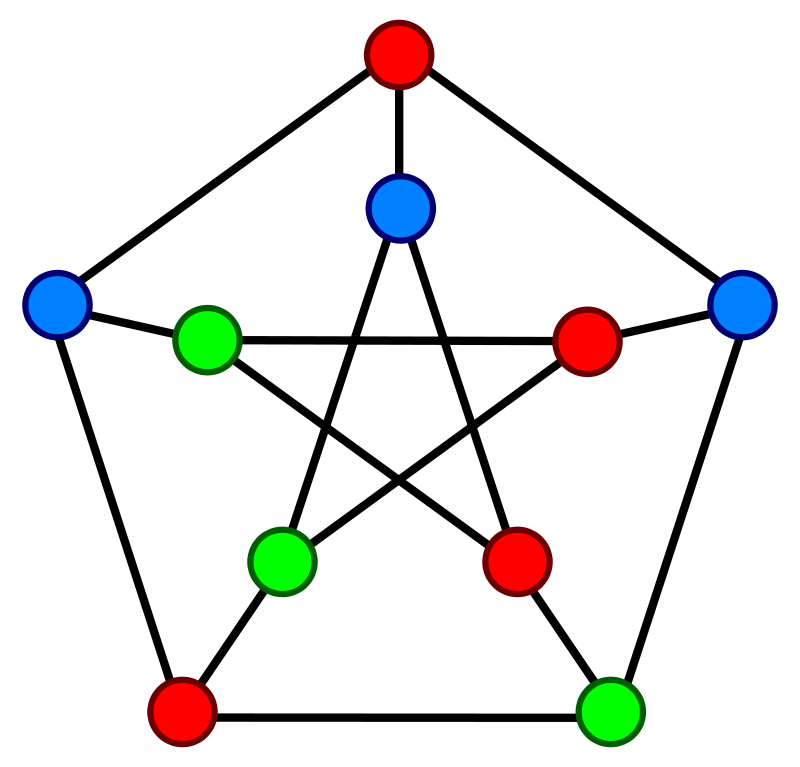
\includegraphics[scale=0.1]{graph-coloring.svg.png}
Имеется граф $G = (V, E)$. Можно ли его вершини расскрасить в $k$ цветов так, чтобы никакие соседние вершины не были раскрашены
в один и тот же цвет?
\end{frame}

\begin{frame}{Раскраска графа}
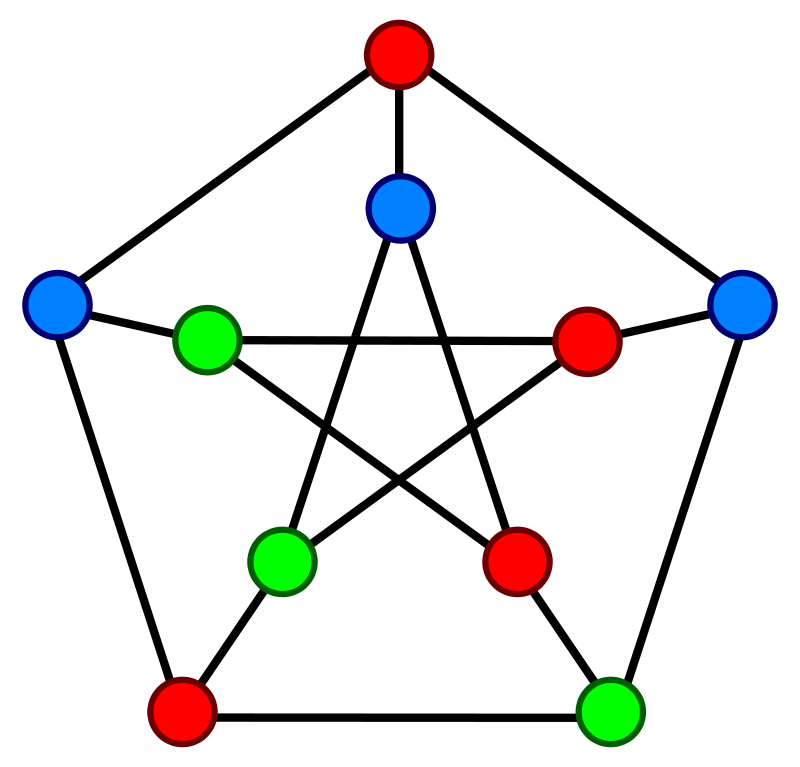
\includegraphics[scale=0.1]{graph-coloring.svg.png}
Имеется граф $G = (V, E)$. Можно ли его вершини расскрасить в $k$ цветов так, чтобы никакие соседние вершины не были раскрашены
в один и тот же цвет?\newline
\begin{itemize}
\item $x_i$ - целые
\item $1 \le x_i \le c$
\item $x_i \neq x_j$ для $(x_i, x_j) \in E$
\end{itemize}
\end{frame}

\begin{frame}{Судоку}
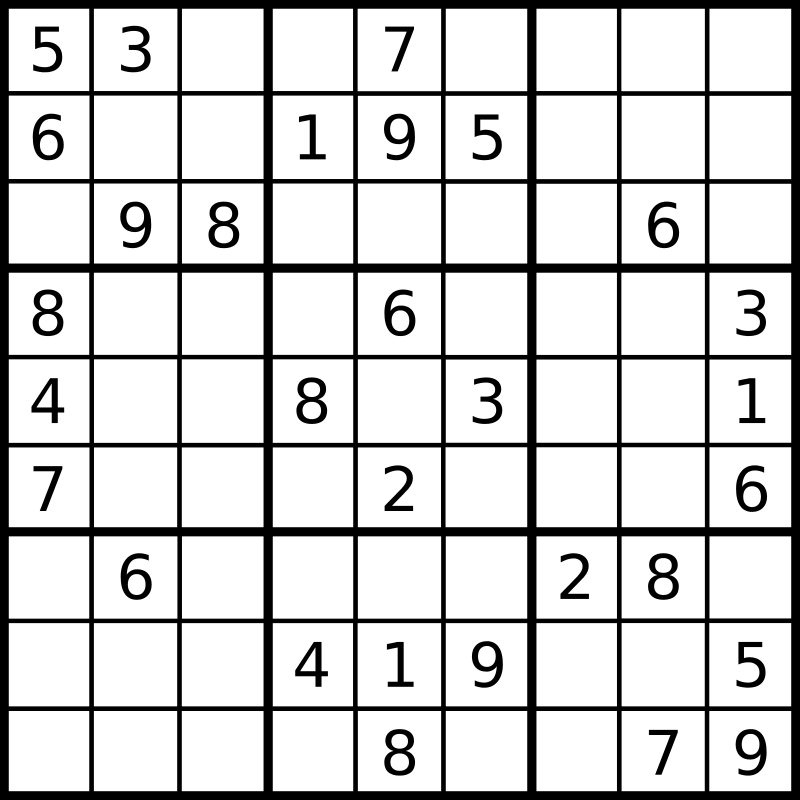
\includegraphics[scale=0.2]{Sudoku.svg.png}
\end{frame}

\begin{frame}{Сапер}
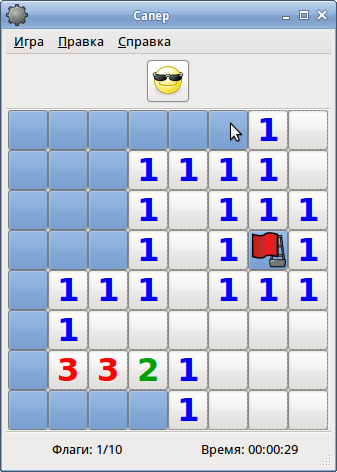
\includegraphics[scale=0.4]{Mines.png}
\end{frame}

\begin{frame}{Эквивалентность программ}
Программа a:\newline
int i, out\_a = in;\newline
for (int i = 0; i < 2; ++i) out\_a = out\_a * inn;\newline
return out\_a;\newline
Программа b:\newline
int out\_b = (in * in) * in;\newline
return out\_b;
\end{frame}

\begin{frame}{Эквивалентность программ}
Программа a:\newline
int i, out\_a = in;\newline
for (int i = 0; i < 2; ++i) out\_a = out\_a * in;\newline
return out\_a;\newline
Программа b:\newline
int out\_b = (in * in) * in;\newline
return out\_b;\newline
$\phi_a := (out\_a_0 = in\_a_0) \wedge (out\_a_1 = out\_a_0 * in\_a_0) \wedge (out\_a_2 = out\_a_1 * in\_a_0)$\newline
$\phi_b := out\_b_0 = (in\_b_0 * in\_b_0) * in\_b_0$\newline
\end{frame}

\begin{frame}{Эквивалентность программ}
Программа a:\newline
int i, out\_a = in;\newline
for (int i = 0; i < 2; ++i) out\_a = out\_a * in;\newline
return out\_a;\newline
Программа b:\newline
int out\_b = (in * in) * in;\newline
return out\_b;\newline
$\phi_a := (out\_a_0 = in\_a_0) \wedge (out\_a_1 = out\_a_0 * in\_a_0) \wedge (out\_a_2 = out\_a_1 * in\_a_0)$\newline
$\phi_b := out\_b_0 = (in\_b_0 * in\_b_0) * in\_b_0$\newline
Чтобы программы были эквивалентны, должно выполняться:\newline
$(in\_a_0 = in\_b_0) \wedge \phi_a \wedge \phi_b \rightarrow out\_a_2 = out\_b_0$
\end{frame}

\begin{frame}
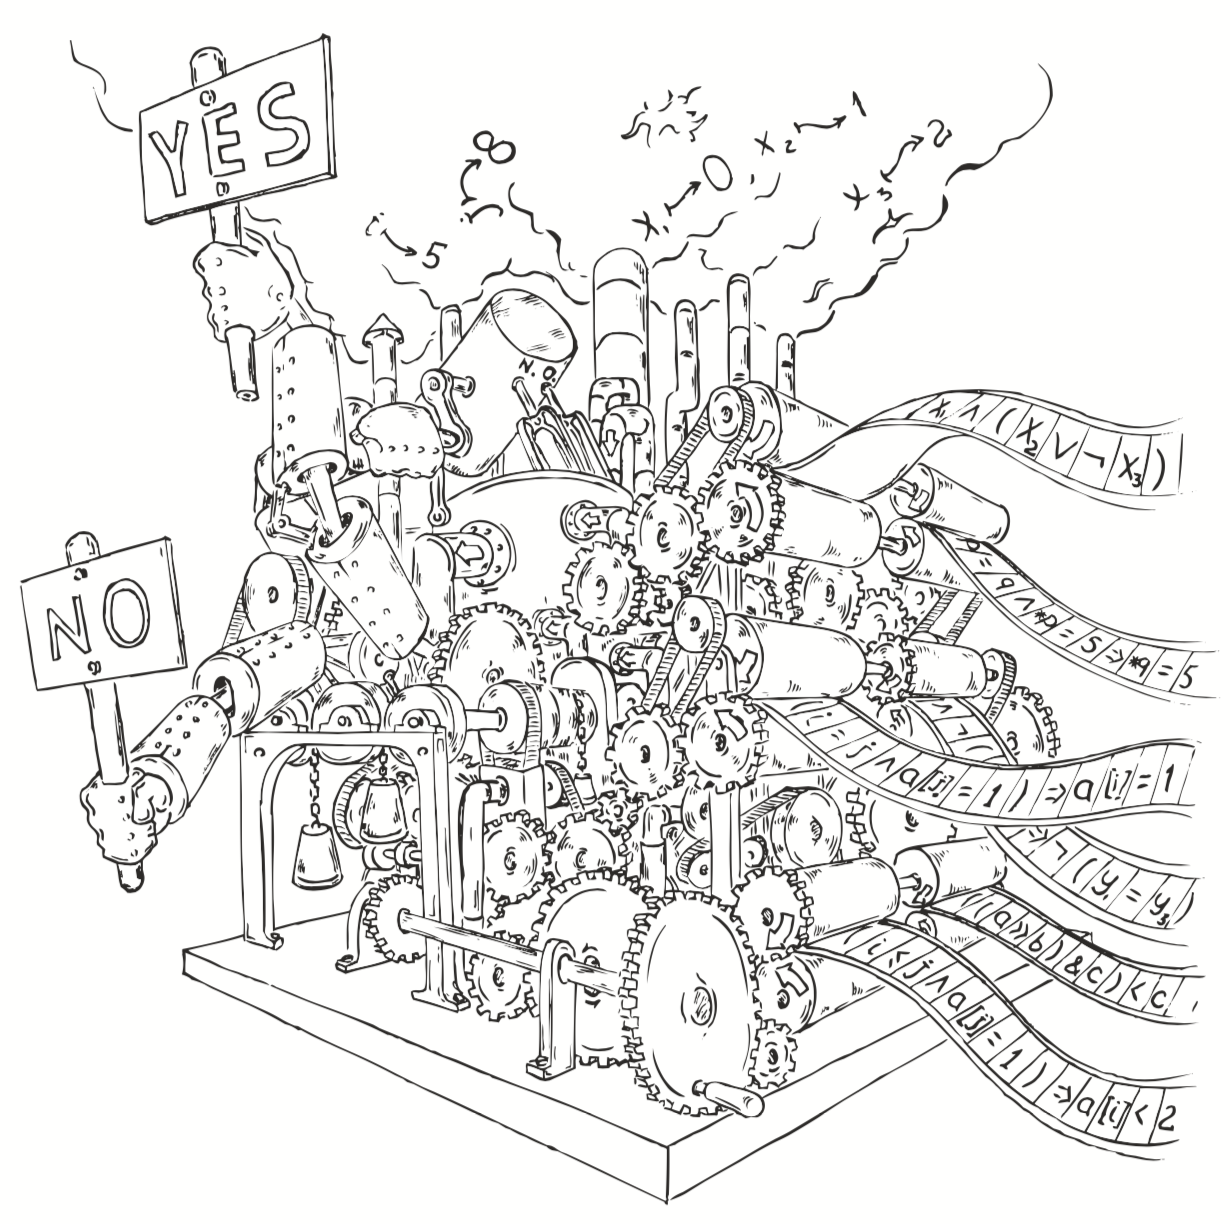
\includegraphics[scale=0.5]{../decision-procedure.png}
\end{frame}

\end{document}
